Using section formula,
\begin{align}
\vec{R}=\frac{1}{1+\frac{1}{2}}\brak{\myvec{4\\-1}+\frac{1}{2}\myvec{-2\\-3}}
=\myvec{2\\ \frac{-5}{3}}\\
\vec{S}=\frac{1}{1+\frac{2}{1}}\brak{\myvec{4\\-1}+\frac{2}{1}\myvec{-2\\-3}}
=\myvec{0\\ \frac{-7}{3}}
\end{align}
which are the desired points of trisection.  See
		\figref{fig:chapters/10/7/2/2/Figure}
\begin{figure}[H]
\centering
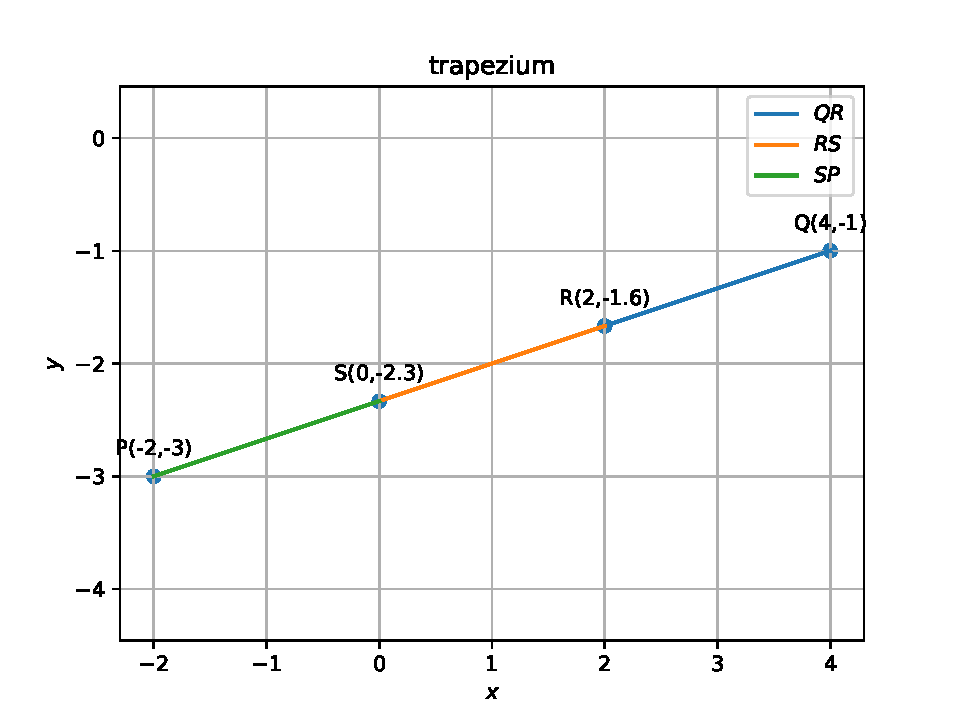
\includegraphics[width=0.75\columnwidth]{chapters/10/7/2/2/figs/dj.pdf}
\caption{}
		\label{fig:chapters/10/7/2/2/Figure}
\end{figure}
